\chapter{Project Design and Development}


\section{System Overview}

The hardware of this vital signs monitoring system has been divided into three major sections as seen in Figure 3.1, namely: 

\begin{itemize}
	\item Sensors - Collects raw measurements of separate vital sign parameters 
	\item Terminals - Processes data and handle transmission/reception of information
	\item Display - Visualises output of critical vital sign information
\end{itemize}

A block diagram of the Wireless Vital Signs Monitoring System is shown in Figure \ref{system} down below. The system consists of three major portions: the Sensors which collect the raw measurements of separate vital sign parameters, the Terminals which process the data and handle transmission/reception of information, and the Display which visualises the output. The details of the development and options considered for each portion are further described in Sections \ref{terminals}, \ref{sensors}, and \ref{processing}.

\begin{figure}[H]
	\centering
	\includegraphics[width=\linewidth]{system2.png}
	\caption{Wireless Vital Signs Monitoring System Block Diagram}
	\label{system}
\end{figure}

\section{Design Specifications}
\label{specifications}

\begin{enumerate}
	\item	The sensors must be able to measure the specified anaesthesia parameters at a basic level. 
	\item 	The following anaesthesia parameters should be monitored: 
	\begin{enumerate}
		\item Electrocardiography (ECG)
		\item Electroencephalography (EEG)
		\item Photoplethysmography (PPG)
		\item Blood Pressure
		\item Blood Temperature 
	\end{enumerate}
	\item	The terminal must be able to process the inputs from the sensors. 
	\item	The terminal must be able to visualise and display the input from the sensors. 
	\item	The terminal must be able to wireless transmit the required information to another display. 
	\item 	The visualised output must be displayed on a monitor. 
	\item	The wireless system must be robust to disconnections due to extended range. 
\end{enumerate}

\section{Actual System Implementation}

\begin{figure}[H]
	\centering
	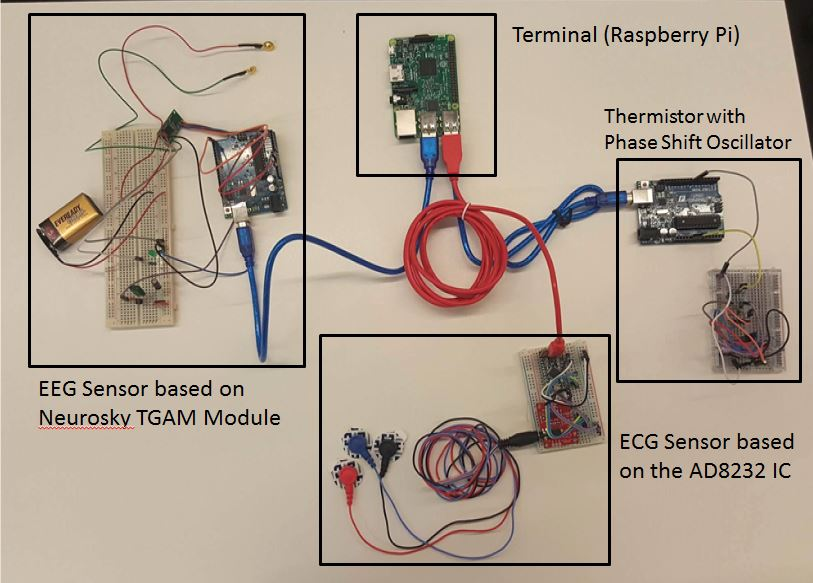
\includegraphics[width=\linewidth]{entiresystemlabelled.jpg}
	\caption{Actual System Implementation of Sensors and Terminal}
\end{figure}